Les opérations de cette phase ont pour but d'extraire les caractéristiques des textes collectés à la phase précédente.
Nous allons rechercher des informations numériques sur la forme des messages comme le nombre de mots, de ponctuations, \ldots\\
Enfin, nous appliquerons des techniques de traitement du langage naturel pour travailler sur le fond des corps de mail.


\subsection{Recherche de caractéristiques}
    Durant cette phase, nous allons rechercher les caractéristiques de la forme du texte.
    L'objectif est de voir si l'utilisation de ponctuation, de certaines formes de mots (majuscule/minuscule)
    ou de construction visuelle d'un texte (espace ligne) est différente pour chaque catégorie de mail.\\

    Les messages seront directement extraits de la base mongo utilisée lors de la phase de fouille.
    Chaque message sera analysé individuellement dans une suite de fonction.
    Les étapes de cette phase sont décrites dans le schéma~\ref{fig:Phase2}.

    \begin{figure}[H]
        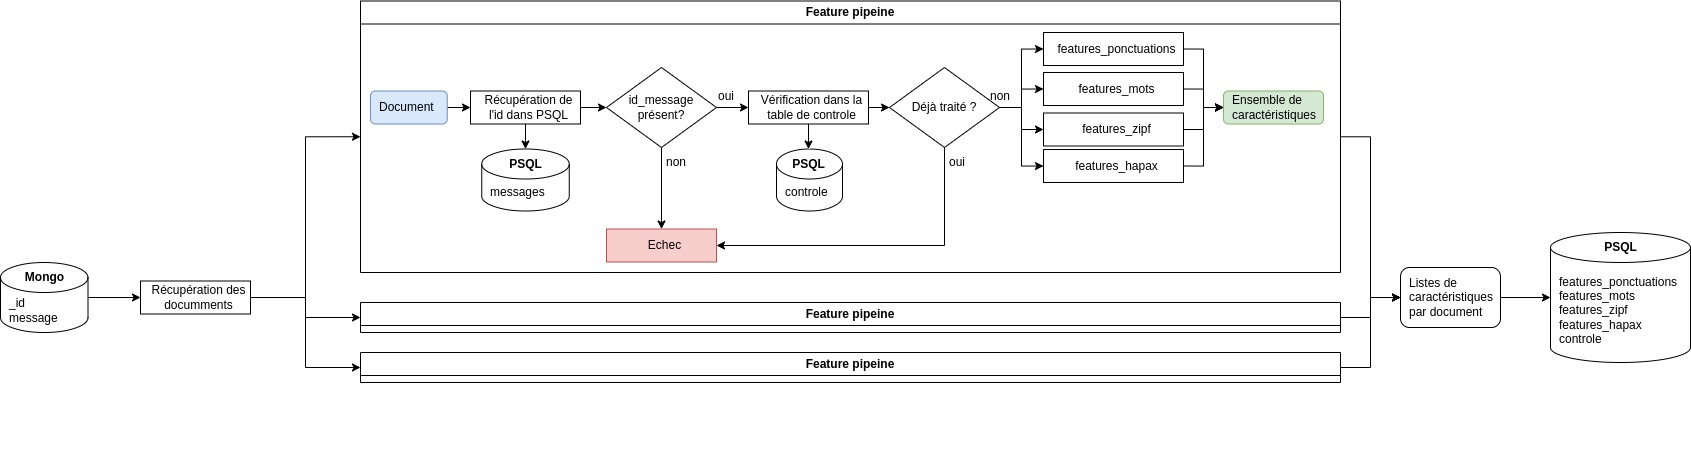
\includegraphics[width=\linewidth]{img/features}
        \caption{Schéma de la recherche de caractéristiques}
        \label{fig:Phase2}
    \end{figure}



    \begin{lstlisting}[title=Fonctions de la recherche de caractéristiques,label={lst:feat_func}]

def features_ponctuations(texte):
    return {
        "point": texte.count('.'),
        "virgule": texte.count(','),
        "exclamation": texte.count('!'),
        "interrogation": texte.count('?'),
        "tabulation": texte.count('\t'),
        "espace": texte.count(' '),
        "ligne": texte.count('\n') + 1,
        "ligne_vide": len(re.findall(r'^\s*$', texte, re.MULTILINE))
    }

ef features_mots(texte):
    tokens = re.findall(r'\w+', texte, re.MULTILINE)
    return {
        'char_minuscules': len(re.findall(r'[a-z]', texte, re.MULTILINE)),
        'char_majuscules': len(re.findall(r'[A-Z]', texte, re.MULTILINE)),
        'mots': len(tokens),
        'mots_uniques': len(set(tokens)),
        'mots_majuscules': sum(mot.isupper() for mot in tokens),
        'mots_capitalizes': sum(bool(re.match(r'[A-Z][a-z]+', mot)) for mot in tokens)
    }


def features_zipf(texte):
    tokens = re.findall(r'\w+', texte, re.MULTILINE)
    z_data = zipf.zipf_process(tokens)
    return {
        'constante': float(z_data.get('const_moy')),
        'coefficient': float(z_data.get('coef_min')),
        'taux_erreur': float(z_data.get('cout_min'))
    }


def features_hapax(texte):
    tokens = re.findall(r'\w+', texte, re.MULTILINE)
    data = zipf.hapax(tokens)
    data['nombre_hapax'] = data.pop('nombres')
    return data
    \end{lstlisting}

    \subsubsection*{Choix technologiques}
        \paragraph{Traitements}
            La recherche des caractéristiques de ponctuations, de type de char, ou de lignes est faite en utilisant la fonction
            standard \emph{str.count()} et le module \emph{re}.\\

            Cette suite de traitement intègre également des fonctions pour le calcul de la distribution de Zipf (annexe~\ref{sec:devZipf}).
            Cela étant, il est possible que les messages soient trop court pour que ces fonctions donnent des résultats pertinents.\\

            L'ensemble des messages sont récupérés dans la base mongo en une seule fois avec l'\_id correspondant au hash.
            Le traitement est effectué sur chaque document en utilisant le module multiprocessing.

        \paragraph{Base de données}
            Les données des documents sont stockées dans des nouvelles tables PSQL initialisées au début du programme.
            Le nouveau schéma PSQL est montré dans la figure \ref{fig:feat_db}
            Cette base a été choisie pour bénéficier des capacités d'insertion par lots et de jointure offertes par SQL\@.
            Plusieurs tables sont ajoutées en liaison avec nom de la fonction de traitement.
            Les tables ajoutées :
            \begin{itemize}
                \item features\_hapax
                \item features\_mots
                \item features\_ponctuations
                \item features\_zipf
            \end{itemize}
            \begin{figure}[H]
                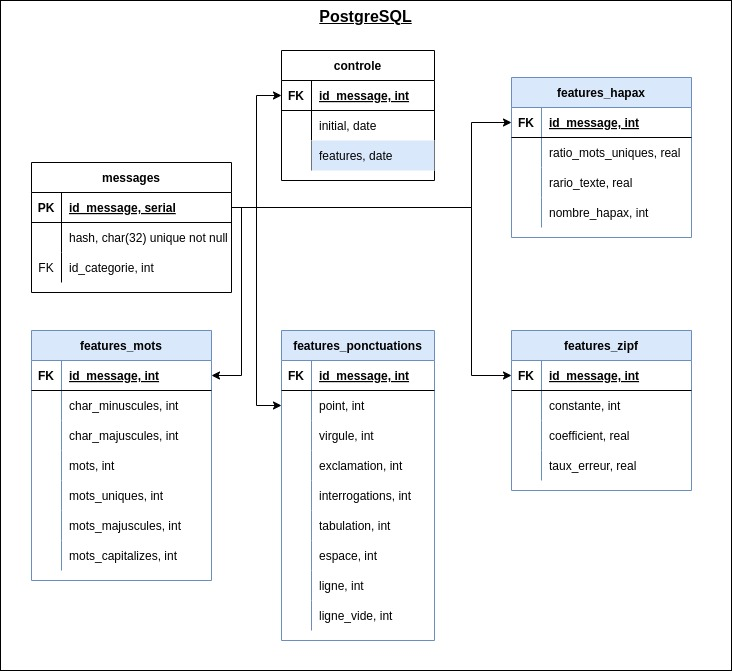
\includegraphics[width=\linewidth]{img/features_bdd}
                \caption{Schéma de la base pour la recherche de caractéristiques}
                \label{fig:feat_db}
            \end{figure}

    \subsubsection*{Analyse partielle}
    TODO

\subsection{Traitement du langage}
    Dans cette section, nous aborderons les traitements du langage naturel qui vont être employés afin de tenter de
    détecter des similitudes dans les thèmes abordés dans les mails de chaque catégorie.
    Nous allons transformer les messages en un dictionnaire de mot et de fréquence.
    Les données récoltées seront utilisées pour vectoriser les documents avec la méthode TF-IDF\@.

    \subsubsection{Lemmatisation}
        La lemmatisation d'un texte vise à réduire la taille d'un texte en ramenant chaque mot à la forme du mot présente dans le dictionnaire.
        Ce traitement permet donc de compter le nombre d'occurrences d'un mot sans se soucier de sa forme ou des modifications grammaticales appliquées lors de la rédaction du texte.
        A l'issue de ce traitement, nous serons en mesure de connaître les mots les plus utilisés dans les corps des mails et tenter de déterminer les thèmes les plus récurrents.
        Dans ce projet, nous allons utiliser le moteur de lemmatisation de \emph{StandfordNLP}\cite{manning-EtAl:2014:P14-5}\cite{qi2020stanza}
        Les traitements nécessaire pour arriver à une lemmatisation sont :
        \begin{enumerate}
            \item Tokenisation - Séparer les phrases en token. Ici chaque token correspond à un mot ou à une ponctuation.
            \item Multi-Word Token Expansion - Ce traitement n'est pas nécessaire en anglais selon la documentation \emph{Stanza}. Il permet d'étendre un token s'il correspond à une contraction de plusieurs terme. Par exemple en français le terme \emph{du} sera transformé en \emph{de le}.
            \item Part of Speech Tagging - Cette opération vise à marquer chaque mot du texte avec sa position grammaticale dans la phrase qui le contient et va permettre d'effectuer le transfert vers le lexème correspondant.
        \end{enumerate}

        L'initialisation de la pipeline de lemmatisation de Stanza se fait en appelant la classe \emph{Pipeline} avec les arguments de langage et de processus dans l'ordre d'utilisation.
        A cette étape, j'ajoute 2 filtres.
        Le premier va me permettre de ne conserver que les mots avec des lettres.
        La deuxième étape permet de retirer les stopwords en anglais qui ne permettent pas d'analyser le sens du message.\\
        La dernière étape avant la mise en base permet de compter la fréquence de chaque mot dans le texte.
        Le schéma~\ref{fig:nlp} illustre l'enchainement des étapes de cette phase.

        \begin{lstlisting}[title=Pipeline de lemmatisation, language=python]
import nltk
import stanza
from src.annexes import zipf

nltk.download("stopwords")
en_stopwd = set(stopwords.words('english'))
pipe = stanza.Pipeline(lang='en', processors='tokenize,mwt,pos,lemma')
pat = re.compile(r'\w+')

def lemmatise(message, stopwds, pipeline, pattern):
    doc = pipeline(message)
    lemma = [mot.lemma for phrase in doc.sentences for mot in phrase.words]
    return [lem.lower() for lem in lemma if re.match(pattern, lem) and lem.lower() not in stopwds]

zipf.freq_mot(lemmatise(value, en_stopwd, pipe, pat))
			\end{lstlisting}

			Ci-dessous un exemple des étapes du traitement sur un message de la base
			\begin{verbatim}
>>> print(value)
Heres the hottest thing in DVDs. Now you can make a personal backup
copy of a DVD right onto CDR.  Our Hot new software easily takes you through
the steps to make a copy of your own DVDs.
NOW INCLUDED FOR FREE! Copy PLAYSTATION, MUSICMPs and all Software.
 Step by Step Interactive Instructions
 All Software Tools Included On CD
 No DVD Burner Required
 FREE Live Technical Support
  Day Risk Free Trial Available
 FREE Dvd Movie of your choice LIMITED TIME OFFER!
We have All the software you need to COPY your own DVD Movies.
This email has been screened and filtered by our in house OPTOUT system in
compliance with state laws. If you wish to OPTOUT from this mailing as well
as the lists of thousands  of other email providers please visit
ZKZmblanzxaDBmnTTIcorikgl

>>> lemmatise(value, en_stopwd, pipe, pat)
['hot', 'thing', 'dvd', 'make', 'personal', 'backup', 'copy', 'dvd', 'right', 'onto',
 'cdr', 'hot', 'new', 'software', 'easily', 'take', 'step', 'make', 'copy', 'dvd',
 'include', 'free', 'copy', 'playstation', 'musicmps', 'software', 'step', 'step',
 'interactive', 'instruction', 'software', 'tool', 'include', 'cd', 'dvd', 'burner',
 'require', 'free', 'live', 'technical', 'support', 'day', 'risk', 'free', 'trial',
 'available', 'free', 'dvd', 'movie', 'choice', 'limited', 'time', 'offer',
 'software', 'need', 'copy', 'dvd', 'movie', 'email', 'screen', 'filter', 'house',
 'optout', 'system', 'compliance', 'state', 'law', 'wish', 'optout', 'mailing',
 'well', 'list', 'thousand', 'email', 'provider', 'please', 'visit',
 'zkzmblanzxadbmntticorikgl']

>>> zipf.freq_mot(lemmatise(value, en_stopwd, pipe, pat))
{'hot': 2, 'thing': 1, 'dvd': 6, 'make': 2, 'personal': 1, 'backup': 1, 'copy': 4,
 'right': 1, 'onto': 1, 'cdr': 1, 'new': 1, 'software': 4, 'easily': 1, 'take': 1,
 'step': 3, 'include': 2, 'free': 4, 'playstation': 1, 'musicmps': 1,
 'interactive': 1, 'instruction': 1, 'tool': 1, 'cd': 1, 'burner': 1,
 'require': 1, 'live': 1, 'technical': 1, 'support': 1, 'day': 1, 'risk': 1,
 'trial': 1, 'available': 1, 'movie': 2, 'choice': 1, 'limited': 1, 'time': 1,
 'offer': 1, 'need': 1, 'email': 2, 'screen': 1, 'filter': 1, 'house': 1,
 'optout': 2, 'system': 1, 'compliance': 1, 'state': 1, 'law': 1, 'wish': 1,
 'mailing': 1, 'well': 1, 'list': 1, 'thousand': 1, 'provider': 1, 'please': 1,
 'visit': 1, 'zkzmblanzxadbmntticorikgl': 1}
			\end{verbatim}

    \begin{figure}[H]
        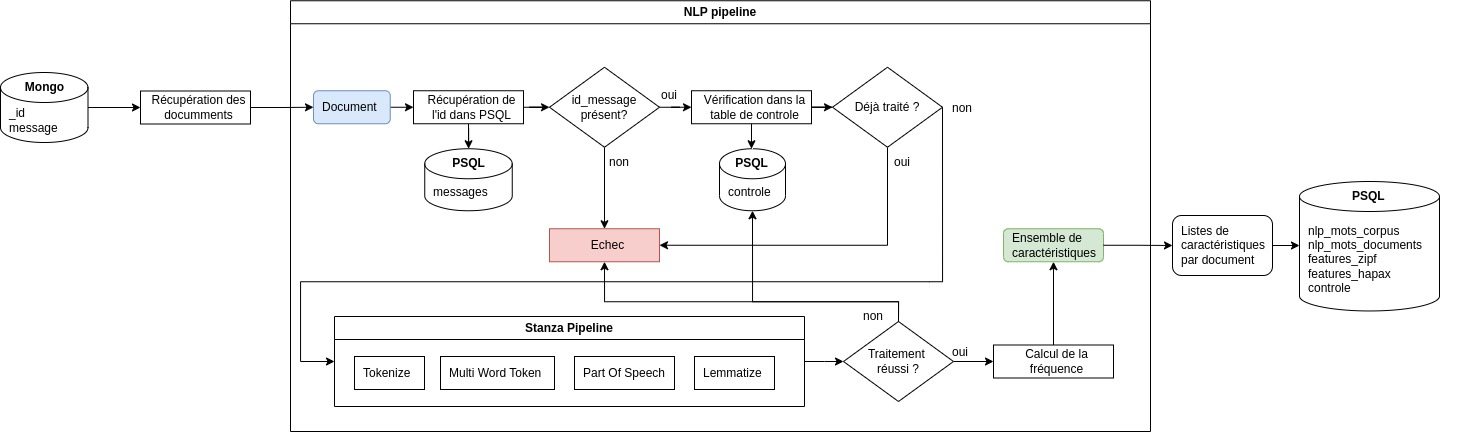
\includegraphics[width=\linewidth]{img/nlp}
        \caption{Schéma du traitement NLP}
        \label{fig:nlp}
    \end{figure}

    \paragraph{Erreurs possibles lors du traitement NLP}
    \begin{itemize}
        \item TypeError - Provient de la présence de données non textuelle dans le corps du mail (ex: MIME)
		\item OutOfMemoryError - Présence de mot beaucoup trop long pour être parsé.
	\end{itemize}

    \paragraph{Choix techniques}
        Seules les librairies de Stanza ont été utilisées pour ce projet pour le traitement de texte.
        J'ai apprécié la simplicité d'intégration de la pipeline dans le code.
        De plus Stanza intègre une capacité de MWT qui aurait pu être utile dans le cas de traitement des mails en français.
        D'autres concurrents sérieux auraient pu être NLTK et SpaCy. Je n'ai pas eu le temps de les approfondir.\\

        Dans cette phase l'utilisation du mutliprocessing n'a pas pu être mis en place à cause d'une RAM limitée qui aurait pu entrainer des échec de traitement.
        De plus, l'utilisation de torch.cuda par la pipeline Stanza nécessite trop d'ajustement au niveau du code pour être utilisées dans ce context.

    \paragraph{Base de données}
        Le schéma de la base de données PSQL pour cette phase est montrée dans la figure~\ref{fig:nlp_db}.
        La table de contrôle récupère 2 nouvelles colonnes
        \begin{itemize}
            \item nlp - date du traitement
            \item nlp\_status - résultat OK, Type error, Memory error
        \end{itemize}

        Deux nouvelles tables sont ajoutées pour stocker les informations nécessaires pour la vectorisation
        \begin{itemize}
            \item nlp\_mots\_corpus - liste des mots présents après les phases de traitement
            \begin{itemize}
                \item freq\_corpus - occurrences du mot dans tout le corpus
                \item freq\_documents - nombre de documents ayant au moins une occurrence de ce mot
                \item freq\_ham - nombre de ham ayant au moins une occurrence de ce mot
                \item freq\_spam - nombre de spam ayant au moins une occurrence de ce mot
            \end{itemize}
            \item nlp\_mots\_documents - liste d'association entre les mots et les documents.
            \begin{itemize}
                \item occurrence - fréquence d'un certain mot dans un document particulier
            \end{itemize}
        \end{itemize}

        \begin{figure}[H]
            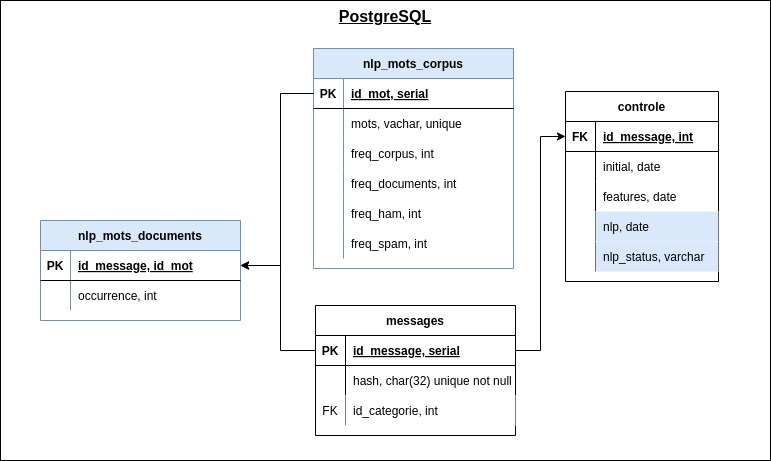
\includegraphics[width=\linewidth]{img/nlp_bdd}
            \caption{Schéma de la base pour le traitement du langage}
            \label{fig:nlp_db}
        \end{figure}

    \paragraph{Analyse partielle}
    TODO

	\subsubsection{Vectorisation}
	    La vectorisation d'un texte doit permettre de transposer les données textuelles en données numériques afin de
        pouvoir les utiliser dans des calculs statistiques ou dans les modèles d'apprentissage automatiques.\\
		J'ai choisi d'utiliser une vectorisation TF-IDF\cite{ml-python} (Term Frequency-Inverse Document Frequency).
        Cette méthode se rapproche de la distribution de Zipf détaillée précédemment.
        En effet, le score d'un terme est dépendant de la fréquence dans le document et de la fréquence de ce terme dans l'ensemble du corpus.
        La formule utilisée est :
        \begin{align*}
            W_{i,j} = tf_{i,j}*log(\frac{N}{df_{i}})
        \end{align*}

        Avec $tf_{i,j}$ la fréquence d'apparition du mot $i$ dans le document $j$, $N$ le nombre de documents dans le corpus et $df_{i}$ le nombre de documents dans le corpus contenant le terme $i$. \\
        Cette méthode permet d'attribuer un score plus élevé aux mots apparaissant plus dans un document que dans les autres documents du corpus.
        Nous pouvons ainsi conserver une forme de contexte d'utilisation.
        La figure~\ref{fig:tfidf} montre les étapes pour vectoriser l'ensemble des documents.

        \begin{figure}[H]
            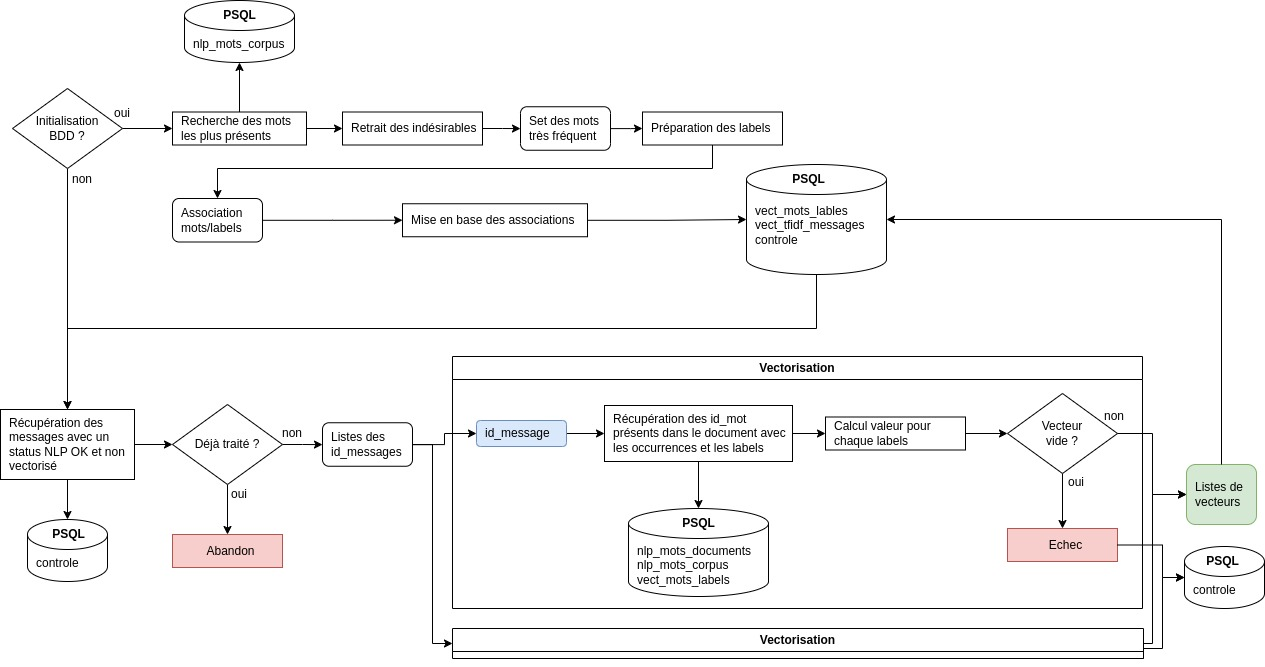
\includegraphics[width=\linewidth]{img/tfidf}
            \caption{Schéma de la vectorisation TFIDF}
            \label{fig:tfidf}
        \end{figure}

        Une fois la phase de récupération des mots faites, il a fallu sélectionner quels mots seront utilisés pour vectoriser les documents.
        J'ai décidé de me limiter sur un ensemble de mots les plus courants dans le corpus sous plusieurs critères :
        \begin{itemize}
            \item Les plus grandes fréquences dans le corpus
            \item Les plus grandes occurrences par catégorie
            \item les occurrences les plus importantes dans les documents d'une catégorie que dans l'autre
        \end{itemize}
        Ces mots sont récupérés via les commandes SQL suivantes :
        \begin{lstlisting}[title=Commandes SQL pour récupérer les mots les plus présent, language=SQL]
SELECT mot FROM nlp_mots_corpus ORDER by freq_corpus DESC;
SELECT mot FROM nlp_mots_corpus ORDER by freq_spam DESC;
SELECT mot FROM nlp_mots_corpus ORDER by freq_ham DESC;
SELECT mot FROM nlp_mots_corpus ORDER by freq_documents DESC;
SELECT mot FROM nlp_mots_corpus ORDER by freq_ham, freq_spam DESC;
SELECT mot FROM nlp_mots_corpus ORDER by freq_spam, freq_ham DESC;
SELECT mot FROM nlp_mots_corpus WHERE freq_ham >= 2*freq_spam ORDER BY freq_ham DESC;
SELECT mot FROM nlp_mots_corpus WHERE freq_spam >= 2*freq_ham ORDER BY freq_spam DESC;
SELECT mot, freq_ham/freq_spam as "ratio ham/spam" FROM nlp_mots_corpus WHERE freq_ham > 0 AND freq_spam > 0 ORDER BY "ratio ham/spam" DESC;
SELECT mot, freq_spam/freq_ham as "ratio spam/ham" FROM nlp_mots_corpus WHERE freq_ham > 0 AND freq_spam > 0 ORDER BY "ratio spam/ham" DESC;
        \end{lstlisting}
        Des \emph{LIMIT X} sont ajoutés à la fin de chaque instruction pour que conserver que les $X$ mots les plus importants.
        Certains mots très fréquents avec une connotation forte sur le dataset ont été retirés (spamassassinsightings, spamassassindevel)
        Le label de chaque mot est construit de la manière suivante, \emph{m\_<id\_mot>}.\\

        Chaque document sera vectorisé en fonction des mots retenus et uniquement avec les informations présentes dans les tables :
        \begin{itemize}
            \item nlp\_mots\_documents(occurrence) - fréquence du mot dans le document
            \item nlp\_mots\_corpus(freq\_documents) - nombre de documents du corpus contenant ce mot
            \item controle(nlp\_status) - count sur le nombre de documents ayant réussi le processus NLP
        \end{itemize}

        \paragraph{Choix techniques}
            Le choix de la vectorisation TFIDF a été décidé par sa proximité avec la distribution de Zipf qui est transposée en python dans ce projet.
            L'idée principale de cette vectorisation était d'avoir un minimum de mots dans la base vectorielle.
            Initialement, j'avais fixé une limite à 200 pour les requêtes SQL\@.
            Cela m'a généré une base d'environ 1200 mots.
            Le problème est que j'ai 5 messages qui ont terminé en vecteur null à la fin de la vectorisation.
            En basculant cette limite à 500 j'obtiens une liste de 2940 mots et tous les documents sont vectorisés.\\

            Le processus de vectorisation utilise également le module multiprocessing pour accélérer au maximum le traitement.
            L'insertion des vecteurs dans la base de données se fait itérativement par document.

        \paragraph{Base de données}
            Le schéma de la base de données pour la phase de vectorisation est montré dans la figure~\ref{fig:tfidf_bdd}.
            \begin{figure}[H]
                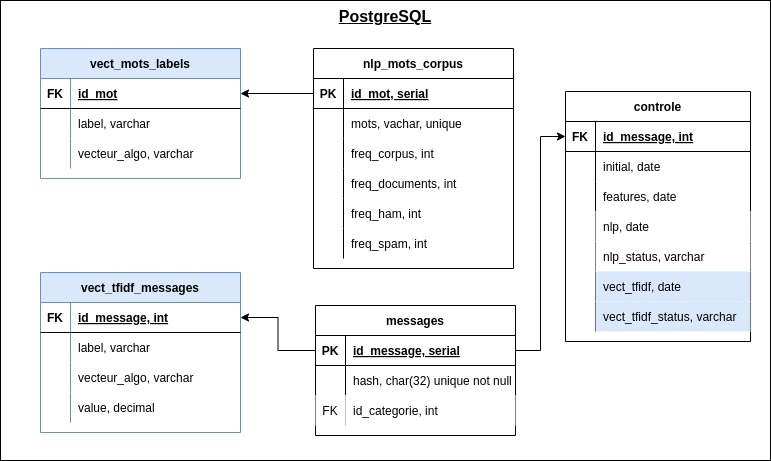
\includegraphics[width=\linewidth]{img/tfidf_bdd}
                \caption{Schéma de la vectorisation TFIDF}
                \label{fig:tfidf_bdd}
            \end{figure}

            Initialement, la table contenant les vecteurs devait avoir comme colonne les labels de chaque mot.
            Cependant, PSQL limite ses tables à 1600 colonnes.
            Ce format aurait dû permettre une intégration plus simple et plus rapide un dataframe pandas pour le traitement via IA\@.\\
            Les tables présentes dans la base sont :
            \begin{itemize}
                \item vect\_mots\_labels - contient la liste d'association entre les mots et les labels définis pour un type de vectorisation
                \item vect\_tfidf\_message - liste toutes les valeurs de la vectorisation par message et par label
                \begin{itemize}
                    \item id\_message
                    \item vecteur\_algo
                    \item label
                    \item value - valeur tfidf pour le message et pour le label
                \end{itemize}
            \end{itemize}
            Cette architecture est plus flexible pour l'ajout de nouvelle méthode de vectorisation.
            Seules les labels non null sont stockés dans la base.
            Cela implique que les labels manquants pour un message doivent être initialisés à 0 avant le début du traitement IA\@.
            La table \emph{vect\_mots\_labels} doit permettre de retrouver la liste complète des labels valident pour un vecteur.

        \paragraph{Analyse partielle}
            TODO